\documentclass{article}
\usepackage{appendix}
\usepackage{graphicx}
\usepackage{pgfplotstable}
\usepackage{listings}
\usepackage{float}

\title{HugeTLB Improvement to Reduce Post-Boot Allocation Failures}
\date{2016-02}
\author{Joshua Nicolas Verburg-Sachs}
\pgfplotsset{compat=1.12}
\begin{document}
	\pagenumbering{gobble}
	\maketitle
	\newpage
	\pagenumbering{arabic}
	\tableofcontents
	\newpage

	\section{Preamble}
		This research was inspired by many frustrated attempts to utilize the excellent huge page facilities of the Linux kernel during runtime. Huge pages are a mechanism whereby the Linux kernel can allocate memory not in 4kb pages (or whatever your distribution uses) but page sizes ranging from many megabytes to a gigabyte or more (though we touch only on the megabyte sized pages in this paper). This gives a variety of advantages, one of the most important being a reduction in the number of page entries that the kernel must manage for your executable. This can, for example, significantly increase the speed of large mmaps and munmaps.

Most of the current use cases and documentation stipulate that you should only attempt to allocate huge pages immediately after boot, in order to avoid (very common) failures due to memory fragmentation and memory use by other executables. However this is not always a convenient option and in some situations (such as real time systems with uptime requirements) it is basically untenable.

Therefore, this paper will describe a method whereby the Linux kernel can be improved to more robustly allocate huge pages during runtime, even when other applications have consumed a significant amount of available memory.

\newpage
\section{Amble}
	There are two primary causes of hugepage allocation failure. In order to illuminate them and discuss the solution we will describe the original algorithm here:
\begin{figure}[h]
\lstinputlisting[firstnumber=967, numbers=left, language=C, firstline=967, lastline=987]{./hugetlb.c.orig}
\label{figure:Original alloc_fresh_huge_page}
\end{figure}

As originally written, the algorithm iterates over the given allowed nodes, calling alloc\_fresh\_huge\_page\_node\footnote{hugetlb.c} which eventually calls into \_\_alloc\_pages\_nodemask\footnote{page\_alloc.c}, where the kernel employs a variety of tools to attempt to enough memory to fulfill the request from this exact node. 

\begin{figure}[h]
...set\_max\_huge\_pages...
\lstinputlisting[firstnumber=1574, numbers=left, language=C, firstline=1574, lastline=1581]{./hugetlb.c.orig}
\label{figure:Excerpt of Original set_max_huge_pages}
...set\_max\_huge\_pages...
\end{figure}

set\_max\_huge\_pages\footnote{hugetlb.c} is called by the kernel to allocate the total requested number of pages. Note that if we fail even a single call of alloc\_fresh\_huge\_page\footnote{hugetlb.c}, we immediately end the attempt to allocate. This can sometimes be worked around by asking the kernel repeatedly to allocate the number of pages, but the allocation will be biased towards the initial nodes searched since we iterate linearly, and eventually they will be exhausted. A situation will quickly arise where the allocation of further huge pages is not limited by available memory but instead by specific nodes which cannot be be passed over by the allocation algorithm. Additionally, the code in page\_alloc.c primarily checks the freelist and then eventually wakes the kswapds. However if the system is under load, this is unlikely to be able to provide enough to fulfill a significant request.

\section{Mosey}
To demonstrate the issues with the original algorithm, as above, we provide two figures which describe 6 different scenarios for the default and new allocation method (hereafter called aggressive). The scenarios are a set of configuration options for the test run in question, where a test run is a certan amount of setup and then an allocation request of the kernel. All scenarios were run directly after a complete reboot, against a 64-bit 3.10 linux kernel\footnote{Linux 3.10.0-327.4.5.el7.x86\_64.debug \#22 SMP x86\_64 GNU/Linux}. The figures are of the average of 10 runs\footnote{All run data availble in appendix D}. These scenarios are encoded as the first letter of each option, followed by a number, and are as follows:
\begin{itemize}
	\item (a)ggressive: Whether to use aggressive alloc.
	\item (s)et: The number of pages to allocate. In all of our tests this number was 500, due to the fact that it was near the maximum suppliable by the system and thus demonstrated the problems with large requests best.
	\item (g)rab: Whether to cause the test application to allocate memory (to disrupt hugepage allocation), and how much if so. 0 means none was allocated. This allocation is done in a series of blocks, rather than in one large request, in order to spread the memory allocations to a variety of nodes and to better simulate the real memory allocation patterns of an application.
	\item (i)terations: How many times the test application should attempt to set the number of huge pages. In all test runs this was 10, as it proved sufficient for demonstrating performance.
	\item (r)eset: Whether to re-set the number of hugepages to 0 after each iteration. 0 means do not reset. We ran 4 scenarios which reset and 2 which did not reset. In many real world scenarios an application making a hugepage request that fails will simply want to back off the allocation and attempt it again later, as it needs the complete request to be fulfilled. However it is also possible that the application will be able to incrementally make use of the hugepages or will be designed to re-request until the allocation is fulfilled, which is likely a necessary choice when requesting large allocations even with these changes. Not resetting the hugepages significantly eases the difficulty of fulfilling the allocation request for the kernel, while resetting demonstrates the efficacy of an intermittent allocation workload.
\end{itemize}\

We use these parameters to define our tests in order to simulate a variety of real world use cases. 
\begin{figure}[h!]
	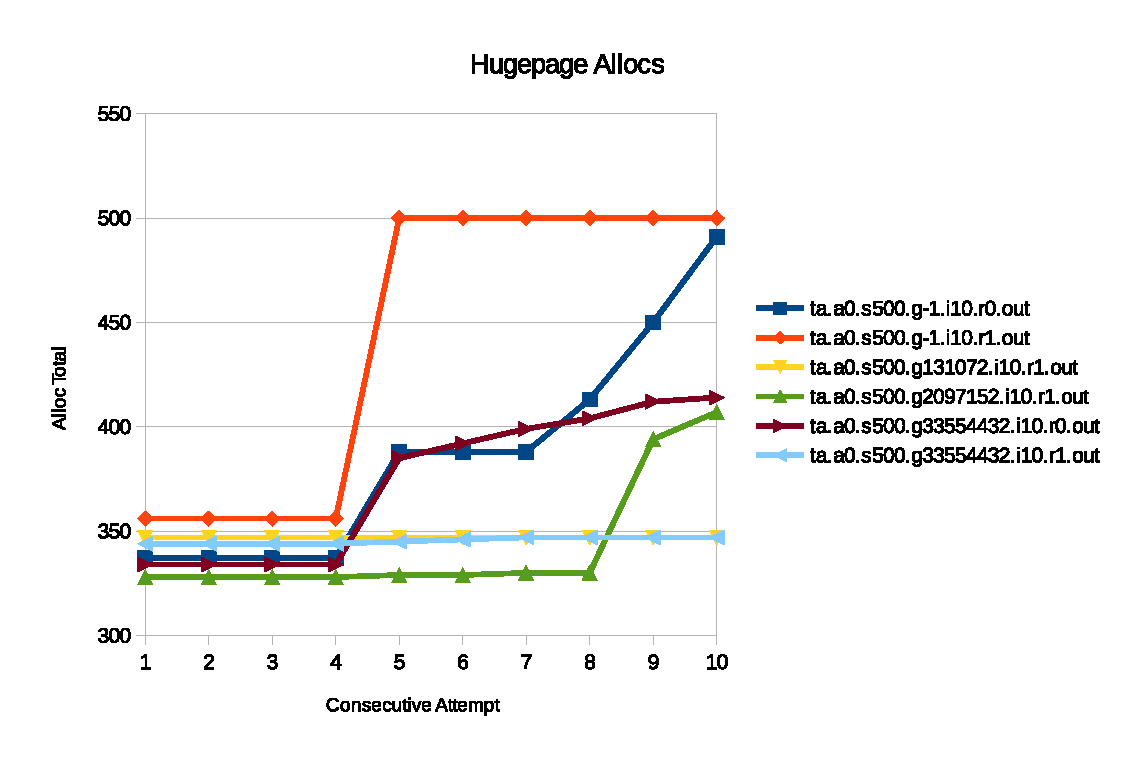
\includegraphics[width=\linewidth]{./datums/default_alloc.eps}
	\label{fig:default_alloc}
\end{figure}

As this chart shows, the default allocation strategy generally fails, on average, to fulfill a large huge page request at runtime. There are three key points on the graph to examine. The first is the initial allocation which for all attempts achieved between 320 and 350 pages of the 500 requested. The next key point is the inflection that occurs at attempt 3 and 4, when all except the most stringent scenario achieved a slightly higher allocation. However, none pass the 400 page mark, and over the course of the next four attempts most barely improve. Much of this improvement can be attributed to anonymous huge pages slowly aggregating all of the memory we are requesting and then re-supplying it to us every time we ask for an allocation. The one scenarion that has not made dramatic improvements is the the g33445532 r1, which is the most demanding scenario. The third key point is the final allocation attempt. At this juncture three scenarios are at about 450 pages (two of which are r0), having improved by roughly 10 pages or so each attempt, though none have completely fulfilled the request. g33554432 r0 has slowly accumulated more pages but is only marginally greater than it was 6 attempts ago, and the two remaining have finally achieved about 400, roughly the same as the 3 best 6 attempts ago. One thing to note is that past success is a strong predictor of future success, as the trend lines demonstrates. In summary, none of these scenarios averaged complete success, and half were at only 400 out of 500 pages after 10 consecutive allocation attemps. Total improvement for the scenarios was capped at roughly 150 pages. Now that we have examined the default scenarios, we will discuss the proposed changes and show the results of the identical tests run against them.

\section{Wander}
There are two important changes to the alloc\_fresh\_huge\_page algorithm. First, if we completely fail to allocate any pages, we call try\_to\_free\_pages\footnote{http://lxr.free-electrons.com/source/mm/vmscan.c\#L2826} (which frees up pages on that node which can be swapped out). If this succeeds, we will once again attempt to allocate on this node. This is important because often allocation on a node is blocked by pages that are still in memory but do not need to be, i.e., they can be swapped out immediately by the kernel. This will effect the performance of other applications on the system but it still follows the default kernel policy (in our case LRU) and therefore disruption should be relatively minimal.

\begin{figure}[H]
\lstinputlisting[firstnumber=1013, numbers=left, language=C, firstline=1013, lastline=1052]{../mm/hugetlb.c}
\label{figure:Aggressive alloc_fresh_huge_page}
\end{figure}

Second, if we succeed in freeing pages then we re-attempt the allocation on that node. Additionally, we made a change to the calling algorithm, set\_max\_huge\_pages, where we will retry until either we succeed in fulfilling the allocation request or we fail at allocating any huge pages twice in a row. Technically we could simply attempt to allocate until there are no available pages left at all, and this would guarantee completion of the request if it is possible, however we decided to make a compromise between efficacy and hogging kernel runtime. An even more relaxed failure tolerance would likely yield even better results but increase the kernel contention significantly.

\begin{figure}[H]
\lstinputlisting[firstnumber=1643, numbers=left, language=C, firstline=1643, lastline=1665]{../mm/hugetlb.c}
\label{figure:Aggressive alloc_fresh_huge_page}
\end{figure}

The next chart shows the difference in success rates for this new strategy. On average, the initial allocation is more than 100 pages higher for all scenarios. Rather than taking 4 consecutive attempts to reliably achieve more than the initial allocation, by the 3rd attempt all scenarios are within 10 pages of their maximum. As can be seen, though only one scenario achieves the total of 500, all scenarios achieve significantly higher allocations significantly faster, with all scenarios above 460 pages at final attempt, which was not achieved by even the least stringent default scenario. Additionally, unlike the default strategy, the scenario configuration had significantly less impact on the success of the allocation, because the aggressive alloc is able to work around large memory allocation and page resets significantly better.  Gathered statistics\footnote{see appendix C} demonstrate the importance of both of the fault tolerance and retry changes we introduced.

\begin{figure}[H]
	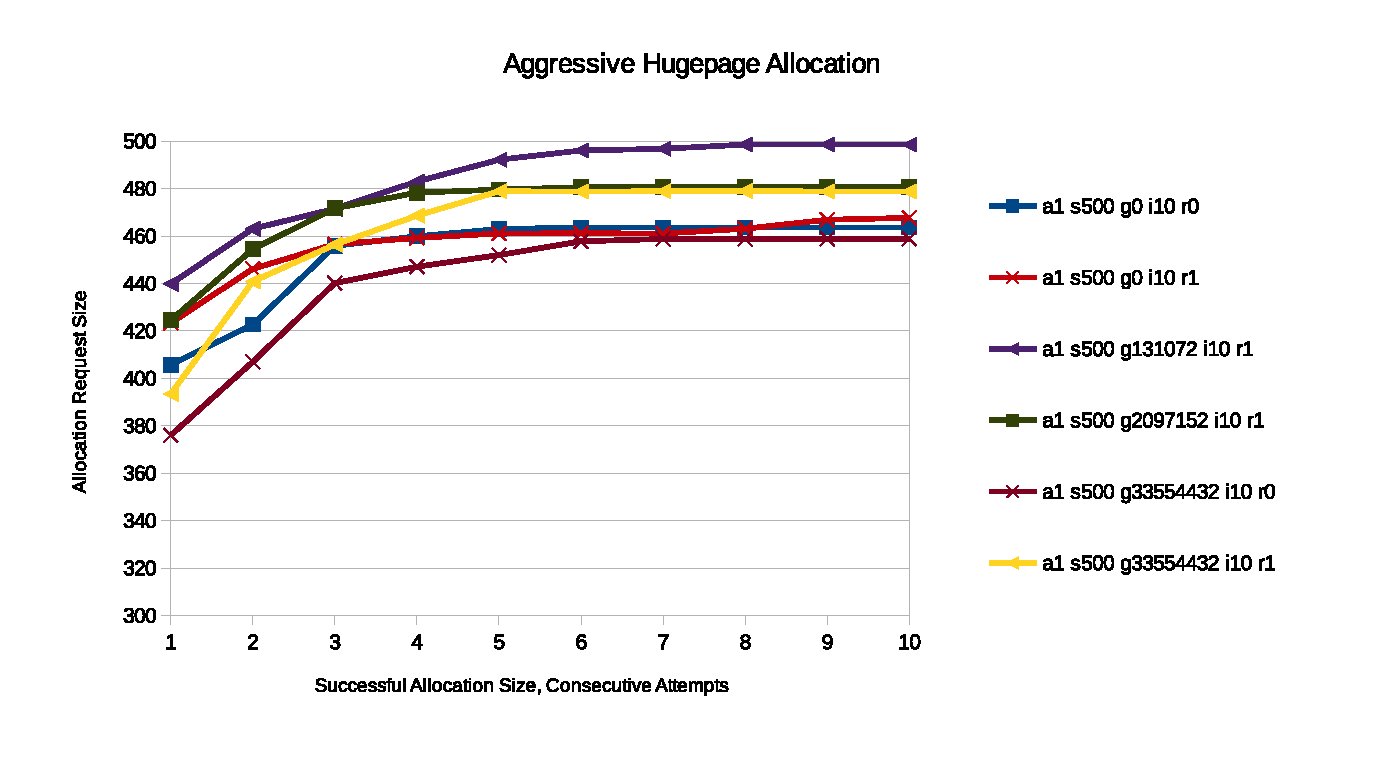
\includegraphics[width=\linewidth]{./datums/aggressive_alloc.eps}
	\label{fig:aggressive_alloc}
\end{figure}

Next, we present a chart of all scenarios' last result to compare ultimate efficacy. Note that scenarios can achieve a maximum result much sooner than the final attempt and in all such cases continued to allocate the maximum number until the end of the scenario. Each column of the chart is the exact same scenario's final result for default and aggressive allocations, for all scenarios run (i.e., 10 runs of each scenario configuration). 46 of 50 of the aggressive scenarios actually completed the 500 page request, but the averages in the charts are lowered by test runs where multiple consecutive nodes are both full and lack enough freeable pages. Conversely, only 3 of 50 the default scenarios achieved 500 pages allocated. Of note is that almost all scenarios for both aggressive and default had at least one test run where the final total failed to achieve a significant improvement over its the initial attempted allocation. We will discuss a potential solution to this issue in Future Works.

\begin{figure}[H]
	\includegraphics[width=\linewidth]{./datums/final_allocs.png}
	\label{fig:final_allocs}
\end{figure}

\section{Future Works}
The one major algorithmic change that could yield even better results than obtained is modifying the set\_max\_huge\_pages algorithm further. Two different strategies could be employed. First, we could avoid the linear search and instead introduce a progressive or randomized starting node choice. This would allow us to eventually overcome a large series of nodes all of which are unusable, however it would place the burden on the requestor to re-ask enough times to fulfill the request. Instead of this, we could make set\_max\_huge\_pages simply skip over unusable nodes until the allocation is completed or it has judged that all suitable nodes are exhausted.

\section{Postamble}
In summary, we have presented a use case for the hugetlb mechanism of the kernel, made changes and demonstrated their efficacy. To do so, we have collected and analyzed data regarding both the current implementation and the aggressive implementation. The data unequivocally show that the new strategy is superior in its ability to fulfill large hugepage allocation requests. We have examined the kernel changes that yielded the results and made suggestions for what could be pursued next. Finally, all data and code used for this paper is available at the public github repository (https://github.com/rivenwyrm/htlb\_project).

\begin{appendices}
	\newpage
	\chapter{Appendix 1: Table}
		\section{Data Table}
		\begin{table}[h!]
			\caption{Hugepage Allocation Data Points}
			\label{table1}
				%some stuff goes here
			\end{table}
	\chapter{Appendix 2: List of Figures}
		\listoffigures
\end{appendices}
\end{document}